\section{Liberalizzazione nelle TLC: primo corpus normativo comunitario}
La concorrenza mette in gioco dinamiche del tipo "se non c'è un'azienda dominante che può fissare un prezzo, ci si orienta verso una riduzione del costo dei servizi forniti da aziende differenti in un mercato liberalizzato". 

La liberalizzazione del mercato è avvenuta sotto la guida europea, per poi diramarsi nei vari Stati: la comunità europea ha a un certo punto stabilito che era lei a gestire determinate problematiche sovranazionali (es. telecomunicazioni).

\subsection{Verso la convergenza tecnologica}
Se vogliamo individuare la causa principale che spinge il meccanismo di innovazione possiamo trovarla nella convergenza tecnologica, ossia il superamento della demarcazione tra mezzi e servizi. 

La branca del diritto che si occupa di questo settore è detta ``diritto della convergenza". 

Durante gli anni '90 si è assistito a numerosi cambiamenti a livello europeo e italiano. La parola telecomunicazioni è presente nella normativa sia italiana che internazionale già nella Convenzione Internazionale di Madrid del 1932. Per telecomunicazioni si intende dunque, tradizionalmente:

\begin{quote}
    Ogni emissione, trasmissione o ricezione di segni, segnali, scritti, immagini, suoni e informazioni di qualsiasi natura, per filo, radioelettrica, ottica o a mezzo di altri sistemi elettromagnetici.    
\end{quote}
(Convenzione Internazionale Madrid 1932, Buenos Aires 1952)

In questa definizione è insita una notevole demarcazione tra i mezzi e i servizi e questo permette alla legislazione che va dagli anni Venti fino alla metà degli anni Ottanta di distinguere strettamente tra mezzi e servizi. 
In un decreto del '73 che regola il codice postale e delle telecomunicazioni si distingue infatti tra:
\begin{itemize}
    \item Telegrafia (via filo)
    \item Telefonia (via filo)
    \item Radiocomunicazioni (onde radio): comprendenti radiodiffusione, radiotelefonia e radiotelegrafia
\end{itemize}

Per gli ambiti di comunicazione One-to-One e comunicazioni broadcast si svilupparono di conseguenza ambiti del diritto distinti.

\begin{figure}
    \centering
    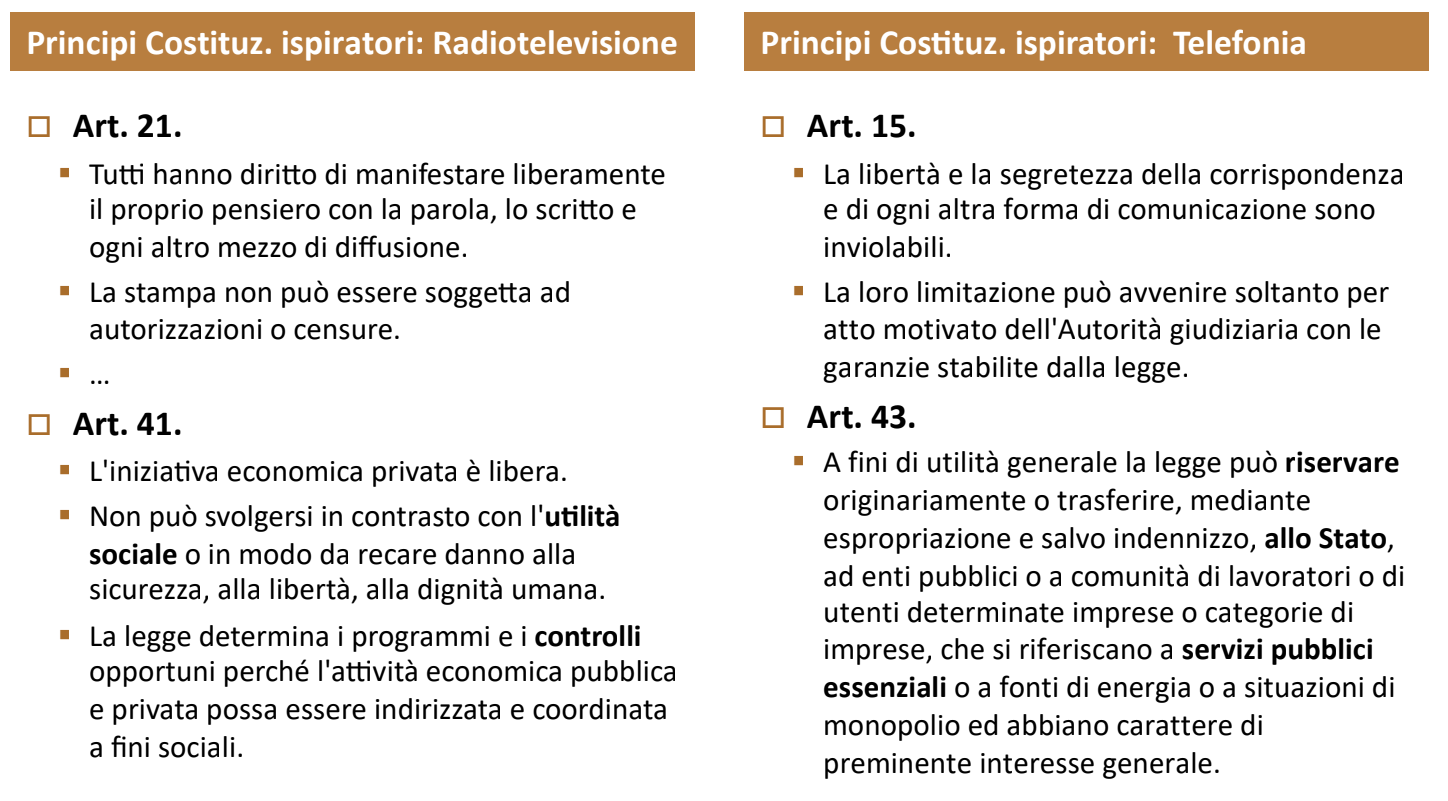
\includegraphics[width=\textwidth]{principi costituzionali.png}
    \caption{Principi costituzionali ispiratori}
\end{figure}

Definiamo \textit{convergenza tecnologica} l'utilizzo stesso mezzo per fornire una pluralità di servizi.

I principali passaggi dell'innovazione tecnologica sono storicamente legati all'avvento della multimedialità:
\begin{itemize}
    \item Telematica: unione tra le TLC e informatica (trasmissione + elaborazione a distanza): l'utente può interagire con l'informazione (anche semplicemente la possibilità di interagire con un televisore tramite telecomando rendendo il servizio non più unidirezionale)
    \item Innovazione e potenziamento dei servizi trasmissivi (fibra, satellite, radiomobile): fruibilità e/o capacità trasmissive notevolmente migliorate
    \item Rappresentazione numerica dell'informazione (segnali): stessa infrastruttura per rappresentare in binario segnali provenienti da diverse sorgenti di informazioni
    \item Sviluppo di tecniche di codifica di sorgente (standard di compressione): riduzione del numero di bit da trasmettere
    \item Tecniche di codifica di canale: affidabilità maggiore della telecomunicazione, riduzione degli errori di trasmissione
    \item Tecniche di crittografia, autenticazione, firma digitale, blockchain: sicurezza, segretezza, autenticazione, privacy, servizi innovativi (es. posta elettronica certificata)
    \item Multimedialità: diverse sorgenti combinate in diversi servizi multimediali su diversi mezzi di tlc collegati attraverso diversi canali di comunicazione in una tendenza alla convergenza di contenuti e servizi su medesime infrastrutture di telecomunicazione
\end{itemize}

Si rese necessario ridefinire delle normative che tenessero conto della multimedialità. 


\subsection{Riflessi dell'innovazione tecnologica sulla disciplina giuridica delle TLC}

\begin{figure}
    \centering
    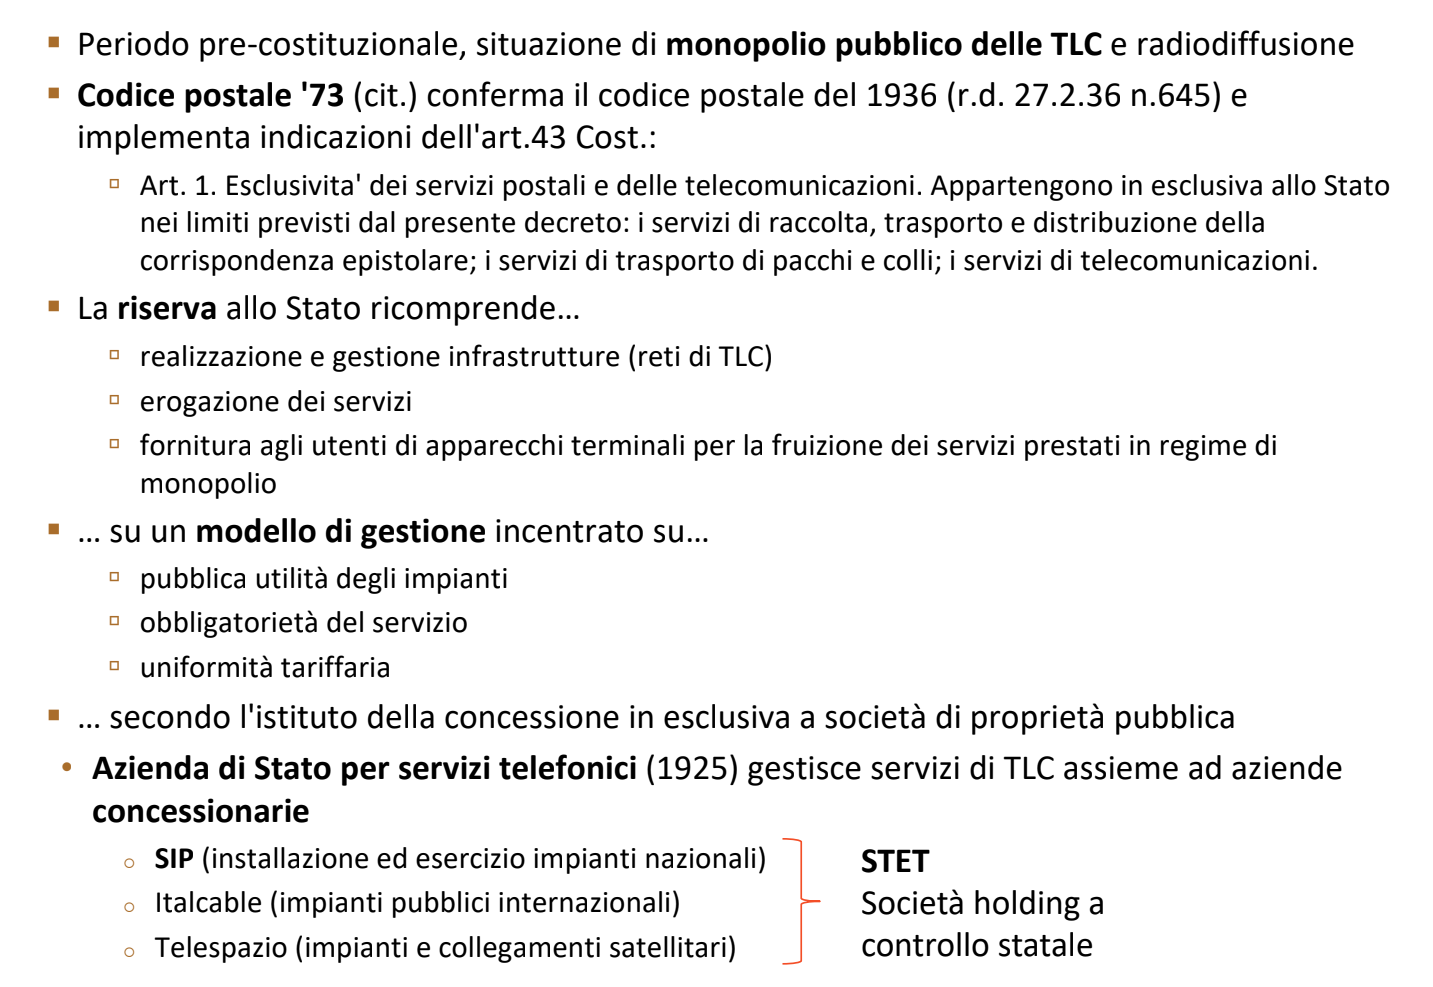
\includegraphics[width=\textwidth]{innovazione tecnologica.png}
\end{figure}


Essendo le problematiche sempre più internazionali (tenendo conto anche della globalizzazione e della mobilità delle persone e delle merci), sempre più decisioni fondamentali vennero prese in sede comunitaria a livello europeo sovranazionale. 

A partire dalla sentenza della Corte di Giustizia del 20/03/1985 su ricorso della Repubblica Italiana vs CE in merito a una sanzione per abuso di posizione dominante a British Telecom ove si respinge il ricorso, si afferma il principio in base al quale le regole della concorrenza sono applicabili anche a organismi pubblici titolari dei diritti esclusivi sulla gestione della rete di telefonia e dei relativi servizi. Ne consegue lo sviluppo di una nuova politica delle TLC a livello europeo volta a:
\begin{itemize}
    \item Liberalizzare i mercati nazionali
    \item Armonizzare le nuove legislazioni nazionali
\end{itemize}

Il processo di regolamentazione comunitaria inizia con il Libro Verde nel 1987 (libro verde sullo sviluppo di un mercato comune dei servizi ed apparati di telecomunicazioni): questo libro trattava della conservazione dei monopoli delle infrastrutture di TLC e della telefonia locale e della liberalizzazione di tutti gli altri servizi. 


ART. 100: sullo stile che la Comunità Europea si dà per cercare di armonizzare e avvicinare i sistemi giuridici dei vari Paesi. 


MAASTRICHT 
ART. 129B: la Comunità concorre alla costituzione e allo sviluppo di reti transeuropee nei settori delle infrastrutture dei trasporti, delle telecomunicazioni e dell'energia. Nel quadro di un sistema di mercati aperti e concorrenziali, l'azione della Comunità mira a favorire l'interconnessione e l'interoperabilità delle reti nazionali, nonché l'accesso a tali reti.

N.B. fino a quel momento i vari Stati avevano sviluppato le proprie tecnologie che non erano compatibili con le tecnologie di altri Stati. Da Maastricht in poi si intraprese un percorso per uniformare le tecnologie in modo da renderle compatibili tra i diversi Paesi.


ART. 129C: la Comunità stabilisce un insieme di azioni per garantire l'interoperabilità delle reti, in particolare nel campo dell'armonizzazione delle norme tecniche

\subsection{Le prime direttive comunitarie: tre fronti di intervento}

Sviluppo tecnologico e grande evoluzione dei ruoli della comunità europea implicano la necessità di una gestione politica della complessità economica. I tre fronti di intervento principali sono:
\begin{enumerate}
    \item Prime parziali liberalizzazioni
    \item Liberalizzazione delle infrastrutture e dei servizi
    \item Interconnessione delle reti e servizio universale 
\end{enumerate}

Questi tre fronti si sviluppano in un primo corpo di direttive comunitarie finalizzato al passaggio dal monopolio alla liberalizzazione del mercato comunitario.

\subsubsection{Prime parziali liberalizzazioni}
\begin{itemize}
    \item Direttiva sui terminali: garantire la concorrenza sui mercati dei terminali di telecomunicazioni, eliminazione dei diritti esclusivi di importazione, commercializzazione e manutenzione dei terminali
    \item Direttiva sulle reti (\textit{Open network provision}): armonizzazione delle condizioni per l'accesso e l'uso libero efficace delle reti pubbliche; in sostanza altri operatori devono poter garantire i propri servizi eventualmente attraverso la rete pubblica senza essere ostacolati
    \item Direttiva sui servizi: liberalizzazione dei servizi di telecomunicazioni a valore aggiunto, stabilisce l'obbligo per gli ex-monopolisti di consentire l'accesso alle proprie reti ai fornitori di servizi liberalizzati. Stabilisce condizioni di accesso eque al mercato concorrenziale (cioè permettere ad altri operatori di accedere senza guadagnarne eccessivamente ma senza nemmeno permettere a chiunque di entrare: introduzione di barriere di accesso al mercato)
\end{itemize}

\subsubsection{Liberalizzazione delle infrastrutture e dei servizi}

Circa 5 anni dopo le prime parziali liberalizzazioni. \
\begin{itemize}
    \item Liberalizzazione delle infrastrutture: si supera la parziale conservazione dei monopoli impostata nel libro verde. Si elimina alcune restrizioni sull'uso di reti televisive via cavo per la fornitura di servizi di tlc già liberalizzati. Viene consentito l'impiego di altre reti cablate per servizi di TLC diversi dai servizi di telefonia vocale e si autorizza l'interconnessione di tali reti alla rete pubblica di TLC. Completa apertura alla concorrenza (\textit{full competition}).
    \item Liberalizzazione dei servizi: armonizzazione delle legislazioni nazionali in merito alla disciplina dei titoli abilitativi
\end{itemize}

\subsubsection{Interconnessione delle reti e servizio universale}

Open network provision: interconnettività a livello logico e fisico tra le reti di tlc in modo che non ci siano incompatibilità.

Nella telefonia c'è stata una fase in cui valeva una parziale interconnessione ma permaneva un problema relativo agli operatori fornitori di servizi (es. per chiamare qualcuno con un operatore diverso era a carico dell'utente l'inserimento di un prefisso opportuno per segnalare la chiamata tra operatori differenti, oppure per cambiare operatore bisognava anche cambiare numero di telefono). 

La politica dell'UE non è quella di espropriare gli stati di un asset importante dal punto di vista economico ma quello di incentivare a privatizzare le aziende e garantire una regolamentazione per gli operatori (dando più diritti ai nuovi entranti nel mercato e più doveri agli ex-monopolisti). 

L'ultima barriera di mercato abbattuta di recente sono le tariffe di roaming per le chiamate internazionali.


Uno dei capisaldi che giustificavano il monopolio era il fatto che si trattasse di servizi che lo Stato doveva garantire a tutti i cittadini indipendentemente dalla posizione geografica agli stessi prezzi in virtù di un principio di equità sociale.

Il principio di equità sociale va coniugato con il contesto in cui i monopoli sono stati distrutti, quindi ecco apparire il concetto di servizio universale.

Servizio universale: insieme minimo definito di servizi, di una data qualità, a disposizione di tu; gli utenti, indipendentemente dalla localizzazione geografica e offerto, in funzione delle specifiche condizioni nazionali, ad un prezzo abbordabile.

Se il servizio universale non porta ricavi sufficienti a compensare la spesa sostenuta per garantirlo, esso viene finanziato attraverso le tasse dei cittadini oppure attraverso un fondo alimentato dagli operatori (secondo regole fissate dagli Stati singolarmente).

\subsection{Caratteristiche di fondo della prima normativa comunitaria}

La politica europea richiede un equilibrio tra la componente politica in sé e la richiesta di regolamentare un ambito (il mondo e il mercato digitali) che dovrebbe in linea teorica rimanere libero da influssi politici, pertanto si è reso necessario applicare un ragionamento orientato alla previsione di possibili sviluppi futuri del mercato digitale.

Se da un lato vediamo aspetti positivi nell'applicazione di una normativa comunitaria (es. privatizzazione dei monopoli statali in virtù di una libertà di mercato) dall'altro si possono verificare casi di eccessiva liberalizzazione. 

Abbiamo visto nella scorsa lezione che sono state introdotte leggi per la liberalizzazione con garanzia di concorrenza, in modo da privatizzare i monopoli statali impedendo che si verifichi un monopolio privato, garantendo dunque l'esistenza della concorrenza. 
Non c'è un'espropriazione dell'infrastruttura di rete in sé, ma si concede che altri soggetti possano contribuire alla realizzazione e gestione di altre reti da introdurre in quella già esistente. 
Lo strumento per riuscire a garantire la concorrenza è la regolamentazione asimmetrica che valuta quali sono gli operatori a più grossa forza di mercato e impone degli obblighi specifici a tali operatori. Per applicare la regolamentazione asimmetrica è necessario avere conoscenza della struttura del mercato di interesse, quindi diventano fondamentali le analisi di mercato. 

Abbiamo visto inoltre il principio del servizio universale, ossia il trasferimento dal monopolista statale alle aziende private dell'obbligo di garantire a tutti i cittadini un servizio minimo. In qualsiasi momento storico ci sarà un insieme di servizi fondamentale per garantire la cittadinanza attiva e, nel caso delle TLC, una vita di relazioni per i cittadini. 

Il servizio universale non necessariamente trova attenzione in un sistema di libero mercato perché da esso non si ricava profitto diretto. Come servizio prevede un meccanismo per cui tutti gli operatori contribuiscono alla garanzia del servizio stesso (eventualmente avvantaggiati da un contributo statale creato attraverso le tasse dei cittadini) attraverso un fondo finalizzato a questo scopo. 

I pubblici poteri diventano un soggetto regolatore del settore supportati dalle normative; la CE ritiene che sia cosa buona che il settore delle TLC sia gestito da autorità indipendenti dalla politica nazionale. In Italia si tratta dell'AGCOM.